\section{Diagramas de Casos de Uso}
	En esta sección se presentan los casos de uso diseñados con base en los RF, RNF y RN. Están ordenados por módulos del sistema.
	\subsection{Módulo de autenticación}
	El módulo de autenticación tiene el siguiente caso de uso que permitirá al usuario autenticarse en la aplicación para poder hacer uso de ésta.
		\subsubsection{CU1: Iniciar sesión}
			\begin{figure}[htbp!]
				\centering
					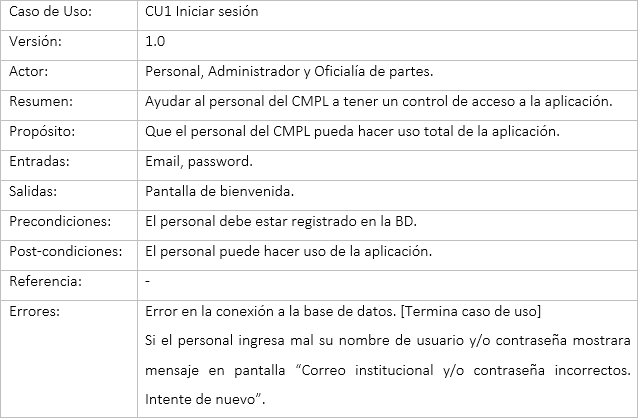
\includegraphics[width=0.8\textwidth]{images/CU/CU1}
					\caption{Caso de uso 1: Inicio de sesión.}
				\label{Tabla}
			\end{figure}
	\subsection{Módulo de Gestión de Usuarios}
	El módulo de Gestión de Usuarios poseé los siguientes casos de uso.
	
		\subsubsection{CU2: Dar de alta empleado del CMPL}
			\begin{figure}[htbp!]
				\centering
					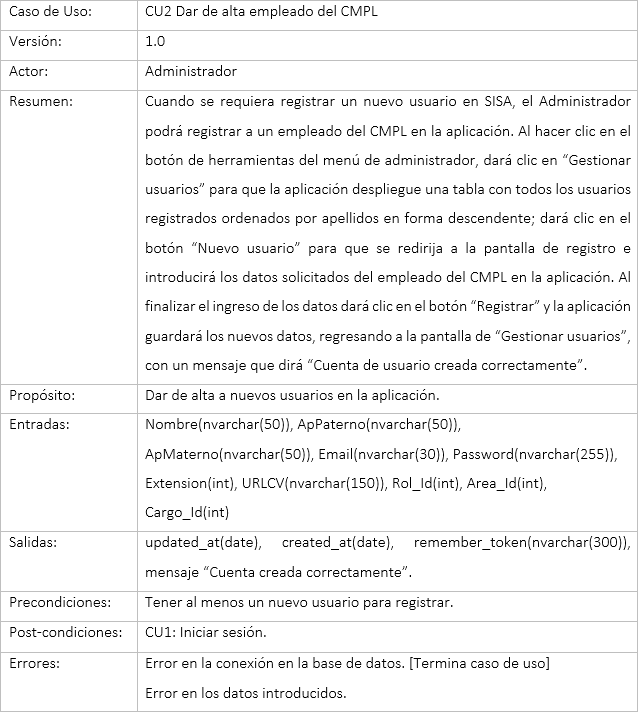
\includegraphics[width=0.8\textwidth]{images/CU/CU2}
					\caption{Caso de uso 2: Dar de alta empleado del CMPL.}
				\label{Tabla}
			\end{figure}
			
			\begin{itemize}
				\item Trayectoria principal:
					\begin{enumerate}
						\item El actor va a la sección de correspondencia 
					\end{enumerate}
				\item Trayectorias alternativas:
					\begin{itemize}
						\item Trayectoria alternativa A:
							\begin{enumerate}
								\item La aplicación muestra un mensaje de error.
							\end{enumerate}
					\end{itemize}
			\end{itemize}
			
		\subsubsection{CU3: Modificar información de un empleado del CMPL}
			\begin{figure}[htbp!]
				\centering
					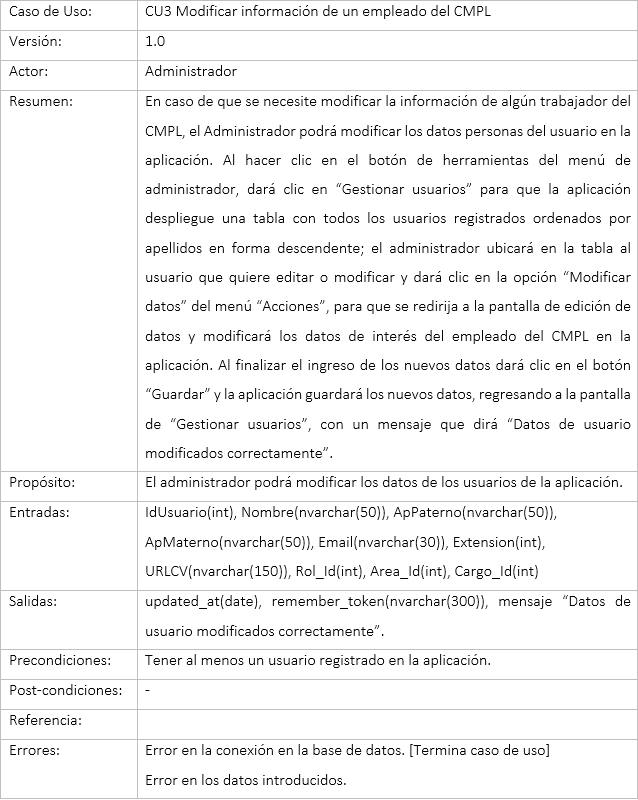
\includegraphics[width=0.8\textwidth]{images/CU/CU3}
					\caption{Caso de uso 3: Modificar información de un empleado del CMPL.}
				\label{Tabla}
			\end{figure}
			
			\begin{itemize}
				\item Trayectoria principal:
					\begin{enumerate}
						\item El actor va a la sección de correspondencia 
					\end{enumerate}
				\item Trayectorias alternativas:
					\begin{itemize}
						\item Trayectoria alternativa A:
							\begin{enumerate}
								\item La aplicación muestra un mensaje de error.
							\end{enumerate}
					\end{itemize}
			\end{itemize}
		
		\subsubsection{CU4: Desactivar cuenta de usuario}
			\begin{figure}[htbp!]
				\centering
					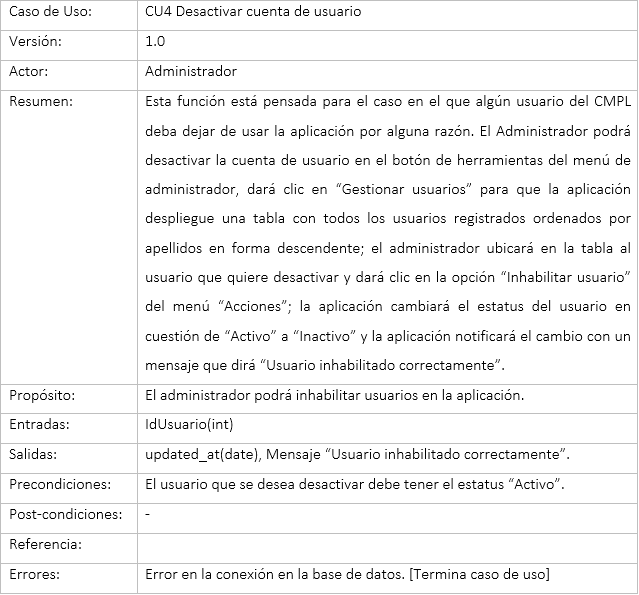
\includegraphics[width=0.8\textwidth]{images/CU/CU4}
					\caption{Caso de uso 4: Desactivar cuenta de usuario.}
				\label{Tabla}
			\end{figure}
			
			\begin{itemize}
				\item Trayectoria principal:
					\begin{enumerate}
						\item El actor va a la sección de correspondencia 
					\end{enumerate}
				\item Trayectorias alternativas:
					\begin{itemize}
						\item Trayectoria alternativa A:
							\begin{enumerate}
								\item La aplicación muestra un mensaje de error.
							\end{enumerate}
					\end{itemize}
			\end{itemize}
			
		\subsubsection{CU5: Activar cuenta de usuario}
			\begin{figure}[htbp!]
				\centering
					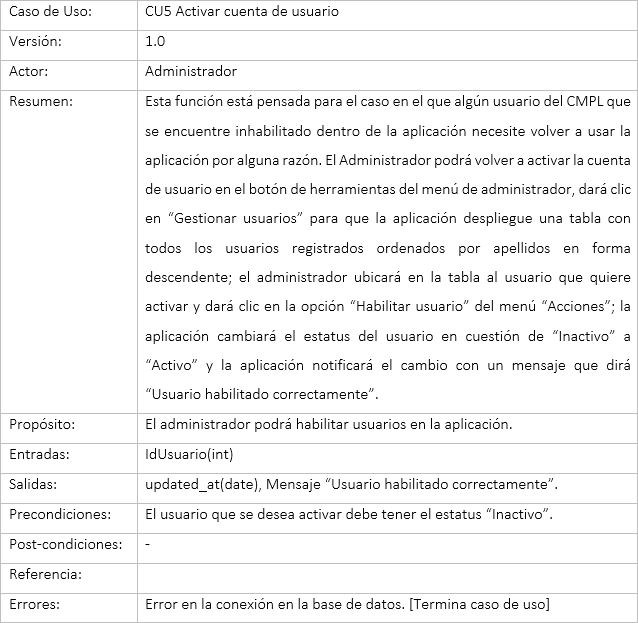
\includegraphics[width=0.8\textwidth]{images/CU/CU5}
					\caption{Caso de uso 5: Activar cuenta de usuario.}
				\label{Tabla}
			\end{figure}
			
			\begin{itemize}
				\item Trayectoria principal:
					\begin{enumerate}
						\item El actor va a la sección de correspondencia 
					\end{enumerate}
				\item Trayectorias alternativas:
					\begin{itemize}
						\item Trayectoria alternativa A:
							\begin{enumerate}
								\item La aplicación muestra un mensaje de error.
							\end{enumerate}
					\end{itemize}
			\end{itemize}
			
		\subsubsection{CU6: Ver directorio interno del CMPL}
			\begin{figure}[htbp!]
				\centering
					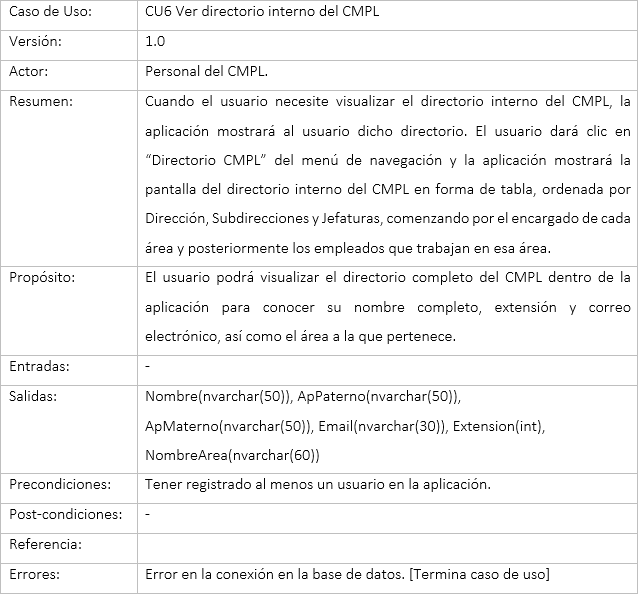
\includegraphics[width=0.8\textwidth]{images/CU/CU6}
					\caption{Caso de uso 6: Ver directorio interno del CMPL.}
				\label{Tabla}
			\end{figure}
			
			\begin{itemize}
				\item Trayectoria principal:
					\begin{enumerate}
						\item El actor va a la sección de correspondencia 
					\end{enumerate}
				\item Trayectorias alternativas:
					\begin{itemize}
						\item Trayectoria alternativa A:
							\begin{enumerate}
								\item La aplicación muestra un mensaje de error.
							\end{enumerate}
					\end{itemize}
			\end{itemize}
			
		\subsubsection{CU7: Ver directorio interno del CMPL por área o departamento}
			\begin{figure}[htbp!]
				\centering
					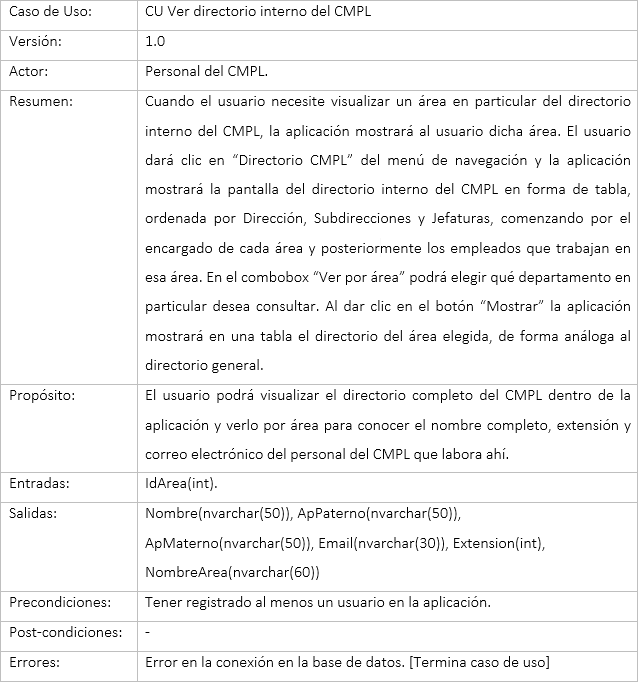
\includegraphics[width=0.8\textwidth]{images/CU/CU7}
					\caption{Caso de uso 7: Ver directorio interno del CMPL por área o departamento.}
				\label{Tabla}
			\end{figure}
			
			\begin{itemize}
				\item Trayectoria principal:
					\begin{enumerate}
						\item El actor va a la sección de correspondencia 
					\end{enumerate}
				\item Trayectorias alternativas:
					\begin{itemize}
						\item Trayectoria alternativa A:
							\begin{enumerate}
								\item La aplicación muestra un mensaje de error.
							\end{enumerate}
					\end{itemize}
			\end{itemize}
			
		\subsubsection{CU8: Buscar empleado del CMPL por nombre}
			\begin{figure}[htbp!]
				\centering
					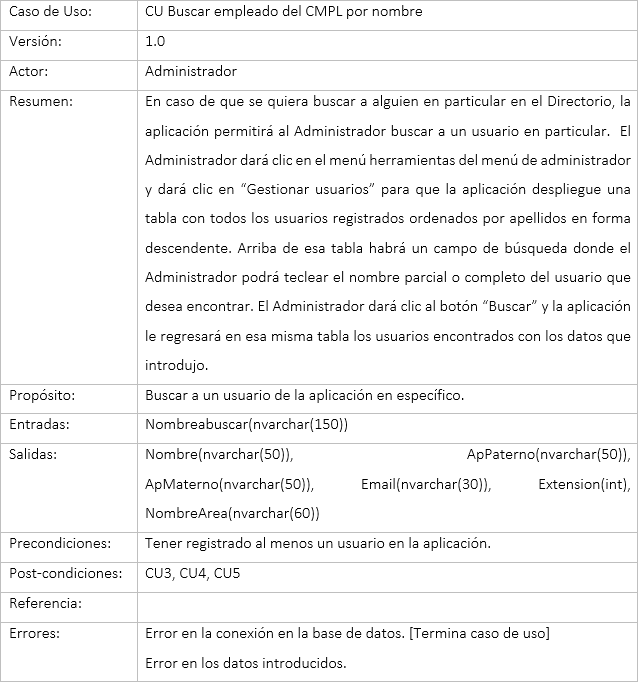
\includegraphics[width=0.8\textwidth]{images/CU/CU8}
					\caption{Caso de uso 8: Buscar empleado del CMPL por nombre.}
				\label{Tabla}
			\end{figure}
			
			\begin{itemize}
				\item Trayectoria principal:
					\begin{enumerate}
						\item El actor va a la sección de correspondencia 
						\item El actor da clic en el menú de herramientas administrativas.
						\item La aplicación muestra el menú de herramientas administrativas.
						\item El actor da clic en la opción ``Gestionar usuarios''.
						\item La aplicación muestra la pantalla \IUref{IU32}, de gestión de usuarios.
						\item El actor introduce en el campo de texto el nombre parcial o completo del usuario que desea localizar y da clic al botón ``Buscar''. 
						\item La aplicación busca en la base de datos el nombre parcial o completo introducido en el campo de búsqueda. \textsl{Trayectoria alternativa A}
						\item La aplicación muestra nuevamente la pantalla \IUref{IU32} con los registros que coinciden en parte o totalmente con los datos ingresados en el campo de búsqueda.

					\end{enumerate}
				\item Trayectorias alternativas:
					\begin{itemize}
						\item Trayectoria alternativa A:
							\begin{enumerate}
								\item La aplicación muestra un mensaje de error.
							\end{enumerate}
					\end{itemize}
			\end{itemize}
			
		\subsubsection{CU9: Restablecer contraseña de usuario}
			\begin{figure}[htbp!]
				\centering
					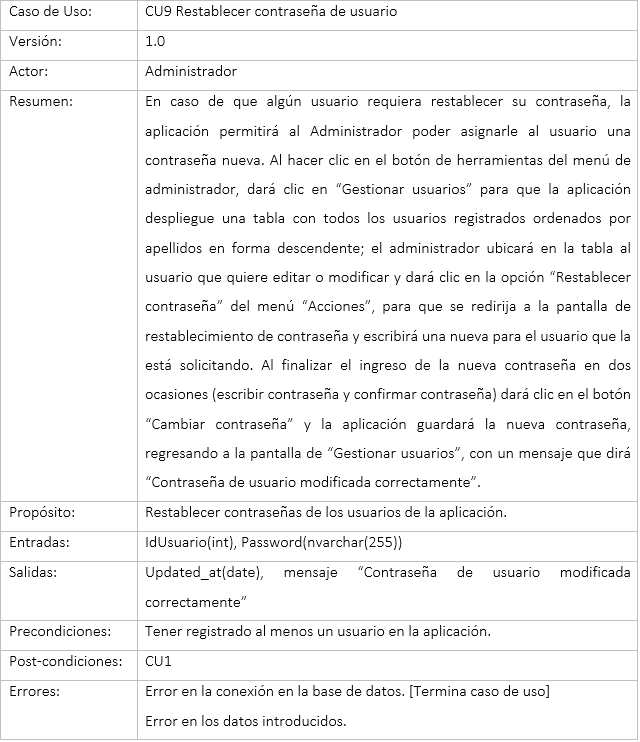
\includegraphics[width=0.8\textwidth]{images/CU/CU9}
					\caption{Caso de uso 9: Restablecer contraseña de usuario.}
				\label{Tabla}
			\end{figure}
			
			\begin{itemize}
				\item Trayectoria principal:
					\begin{enumerate}
						\item El actor va a la sección de correspondencia 
						\item El actor da clic en el menú de herramientas administrativas.
						\item La aplicación muestra el menú de herramientas administrativas.
						\item El actor da clic en la opción ``Gestionar usuarios''.
						\item La aplicación muestra la pantalla \IUref{IU32}, de gestión de usuarios.
						\item El actor elije el usuario que desea editar y da clic al botón ``Acciones'' del menú de opciones de ese usuario.
						\item La aplicación muestra el menú de opciones del usuario seleccionado.
						\item El actor da clic en ``Restablecer contraseña''.
						\item La aplicación muestra la pantalla \IUref{IU36}, de restablecimiento de contraseña.
						\item El actor teclea una nueva contraseña.
						\item El actor vuelve a teclear la nueva contraseña.
						\item El actor da clic al botón ``Cambiar contraseña''.
						\item La aplicación verifica que ambos campos de contraseña coincidan. \textsl{Trayectoria alternativa A}
						\item La aplicación verifica que la contraseña no sea menor a 6 dígitos. \textsl{Trayectoria alternativa B}
						\item La aplicación cambia la contraseña del usuario seleccionado.
						\item La aplicación muestra la pantalla \IUref{IU32}, de gestión de usuarios, con el mensaje ``Contraseña de usuario modificada correctamente''.

					\end{enumerate}
				\item Trayectorias alternativas:
					\begin{itemize}
						\item Trayectoria alternativa A:
							\begin{enumerate}
								\item La aplicación muestra un mensaje de error.
							\end{enumerate}
					\end{itemize}
			\end{itemize}
			
		\subsubsection{CU10: Cambiar contraseña}
			\begin{figure}[htbp!]
				\centering
					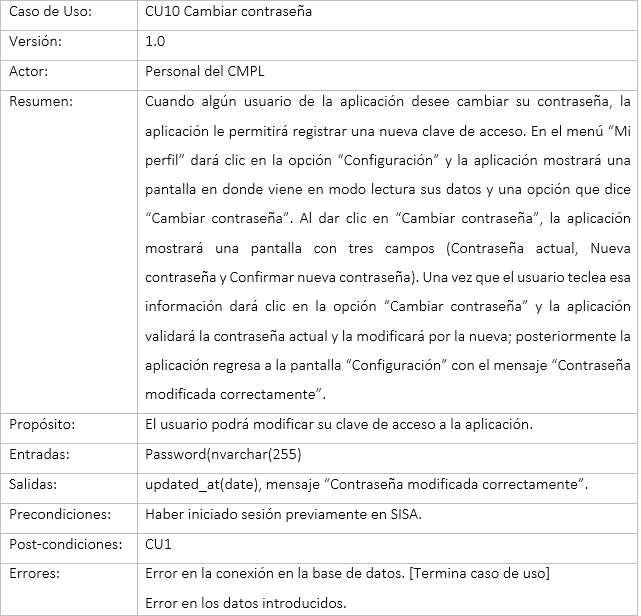
\includegraphics[width=0.8\textwidth]{images/CU/CU10}
					\caption{Caso de uso 10: Cambiar contraseña.}
				\label{Tabla}
			\end{figure}
			
			\begin{itemize}
				\item Trayectoria principal:
					\begin{enumerate}
						\item El actor va a la sección de correspondencia 
						\item El actor da clic en el menú ``Mi perfil''.
						\item La aplicación muestra el menú del perfil de usuario.
						\item El actor da clic en la opción ``Configuración''.
						\item La aplicación muestra la pantalla \IUref{IU37}, de Mi perfil.
						\item El actor selecciona el botón ``Cambiar contraseña''.
						\item La aplicación muestra la pantalla \IUref{IU36}, de restablecimiento de contraseña.
						\item El actor teclea una nueva contraseña.
						\item El actor vuelve a teclear la nueva contraseña.
						\item El actor da clic al botón ``Cambiar contraseña''.
						\item La aplicación verifica que ambos campos de contraseña coincidan. \textsl{Trayectoria alternativa A}
						\item La aplicación verifica que la contraseña no sea menor a 6 dígitos. \textsl{Trayectoria alternativa B}
						\item La aplicación cambia la contraseña del usuario seleccionado.
						\item La aplicación muestra la pantalla \IUref{IU37}, de Mi perfil, con el mensaje ``Contraseña modificada correctamente''.
					\end{enumerate}
				\item Trayectorias alternativas:
					\begin{itemize}
						\item Trayectoria alternativa A:
							\begin{enumerate}
								\item La aplicación muestra un mensaje de error.
							\end{enumerate}
					\end{itemize}
			\end{itemize}


A continuación se muestran los casos de uso para los oficios.

		\subsubsection{CU11: Registrar oficio saliente}
\begin{figure}[htbp!]
		\centering
			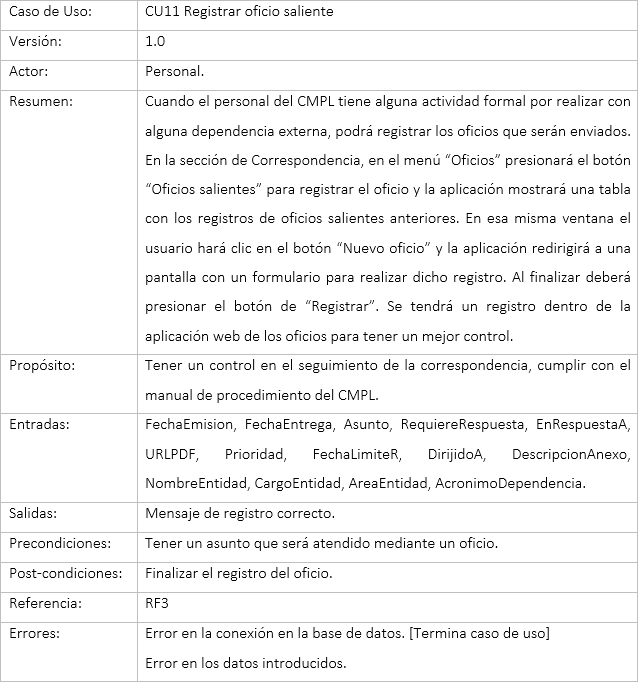
\includegraphics[width=0.8\textwidth]{images/CU/CU11}
		\caption{Caso de uso 11: Registrar oficio saliente.}
		\label{Tabla}
	\end{figure}

\begin{itemize}
	\item Trayectoria principal:
	\begin{enumerate}
		\item El actor va a la sección de correspondencia 
		\item La aplicación muestra la pantalla \IUref{IU21} Correspondencia.
		\item El actor presiona el botón “Nuevo oficio”.
		\item La aplicación muestra la interfaz \IUref{IU10} para el registro de oficios.
		\item El actor introduce los datos requeridos para el registro del oficio.
		\item El actor presiona el botón “Adjuntar documento”.
		\item El actor selecciona el archivo que va a subir.
		\item El usuario presiona el botón “Registrar”. 
		\item La aplicación hace la validación de los datos introducidos. \textsl{Trayectoria alternativa A} 
		\item La aplicación muestra el mensaje \IUref{MSG2} de que el registro se realizó de forma exitosa.
		\item Fin del caso de uso.
	\end{enumerate}
	
	\item Trayectorias alternativas:
	\begin{itemize}
		\item Trayectoria alternativa A:
			\begin{enumerate}
				\item La aplicación muestra un mensaje de error.
				\item La aplicación resalta los campos en el formulario con errores.
				\item El usuario corrige los errores en el formulario.
				\item Continua en trayectoria del CU11 en paso 8.
			\end{enumerate}
	\end{itemize}
\end{itemize}
%%%%%%%%%%%%%%%%%%%%%%%%%%%%%%%%%%%%%%%%%%%%%%%%%%%%%%%%%%%%%%%%%%%%%%%%%%%
		\subsubsection{CU12: Registrar oficio entrante}
	\begin{figure}[htbp!]
		\centering
			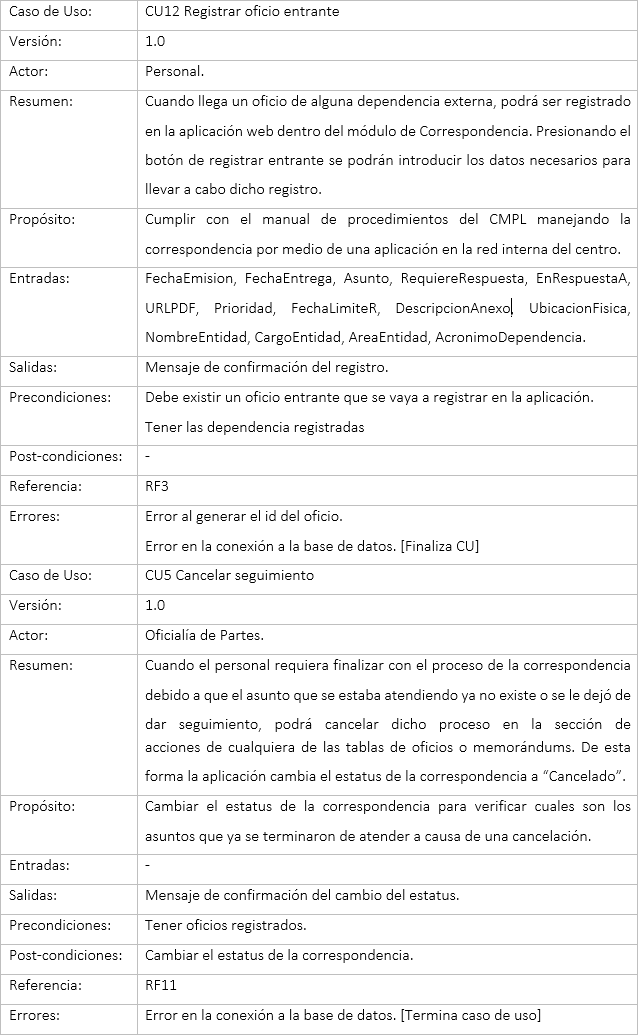
\includegraphics[width=0.8\textwidth]{images/CU/CU12}
		\caption{Caso de uso 12: Registrar oficio entrante.}
		\label{Tabla}
	\end{figure}
	
\begin{itemize}
	\item Trayectoria principal:
	\begin{enumerate}
		\item	El actor va a la sección de correspondencia 
\item	El actor da clic en el botón “Oficios entrantes”.
\item	La aplicación muestra la pantalla \IUref{IU4} Correspondencia Oficios entrantes.
\item	El actor presiona el botón “Nuevo oficio”.
\item	La aplicación muestra la interfaz \IUref{IU9} para el registro de oficios entrantes.
\item	El actor introduce los datos requeridos para el registro del oficio.
\item	El actor presiona el botón “Adjuntar documento”.
\item	El actor selecciona el archivo que va a subir.
\item	El actor presiona el botón “Registrar”.
\item	La aplicación hace la validación de los datos introducidos.
\item	La aplicación muestra el mensaje \IUref{MSG2} de que el registro se realizó de forma exitosa.
\item	La aplicación redirige al usuario a la pantalla \IUref{IU4}.
\item	CU13 Turnar correspondencia.
\item	Termina caso de uso.

	\end{enumerate}
	
	\item Trayectorias alternativas:
	\begin{itemize}
		\item Trayectoria alternativa A: Si los datos introducidos no son válidos.
			\begin{enumerate}
				\item La aplicación web resalta los datos que no fueron introducidos correctamente. 
				\item Regresa a la trayectoria principal en paso 5.
			\end{enumerate}
	\end{itemize}
\end{itemize}

%%%%%%%%%%%%%%%%%%%%%%%%%%%%%%%%%%%%%%%%%%%%%%%%%%%%%%%%%%%%%%%%%%%%%%%%%%%%
		\subsubsection{CU13: Turnan oficio}
\begin{figure}[htbp!]
		\centering
			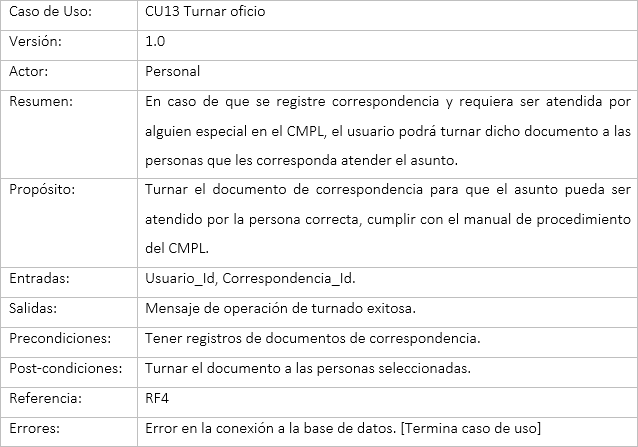
\includegraphics[width=0.8\textwidth]{images/CU/CU13}
		\caption{Caso de uso 13: Turnar oficio.}
		\label{Tabla}
	\end{figure}
	
\begin{itemize}
	\item Trayectoria principal:
	\begin{enumerate}
		\item	El actor va a la sección de correspondencia.
\item	Selecciona el tipo de correspondencia que desea turnar (oficio entrante o saliente, memorándum enviado o recibido).
\item	La aplicación muestra la pantalla \IUref{IU4} Correspondencia correspondiente.
\item	El actor presiona el botón “Acciones” de la correspondencia interesada.
\item	El actor presiona la opción “Turnar a” del documento que desee turnar.
\item	La aplicación muestra la pantalla \IUref{IU38} para turnar correspondencia.
\item	El actor ingresa el nombre en el campo de búsqueda de la persona a la cual desea turnar el documento o la selecciona por departamento y presiona “Buscar”.
\item	La aplicación regresa la pantalla con los resultados de la búsqueda.
\item	El actor presiona el botón “Añadir” del registro de la persona a la que desea turnar el documento.
\item	La aplicación muestra en la pantalla una tabla con los nombres y departamentos de las personas a las que se les indicó como “Añadir” en el paso 9.
\item	El actor da clic en el botón “Turnar correspondencia”.
\item	La aplicación registra dicha operación en la base de datos.
\item	La aplicación muestra el mensaje \IUref{MSG5} de que la operación se realizó con éxito.
\item	Termina caso de uso.

	\end{enumerate}
	
\end{itemize}

%%%%%%%%%%%%%%%%%%%%%%%%%%%%%%%%%%%%%%%%%%%%%%%%%%%%%%%%%%%%%%%%%%%%%%%%%%%%
		\subsubsection{CU14: Guardar acuse}
\begin{figure}[htbp!]
		\centering
			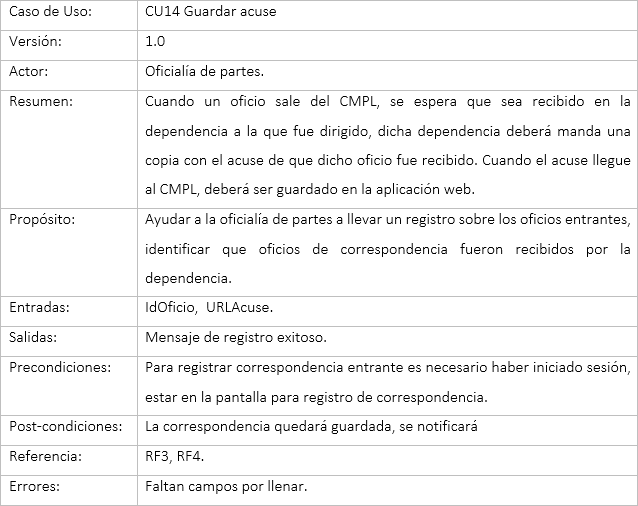
\includegraphics[width=0.8\textwidth]{images/CU/CU14}
		\caption{Caso de uso 14: Guardar acuse.}
		\label{Tabla}
	\end{figure}
	
\begin{itemize}
	\item Trayectoria principal:
	\begin{enumerate}
		\item 	El actor va a la sección de correspondencia.
\item	El actor selecciona en el menú “Oficios” la opción “Oficios salientes”.
\item	La aplicación muestra la pantalla \IUref{IU21} Correspondencia Oficios salientes.
\item	El actor da clic en el botón “Adjuntar documento”.
\item	El actor da clic en el botón “Subir”.
\item	La aplicación guarda en el Servidor el documento PDF y registra su ruta de acceso en la BD.
\item	La aplicación muestra la pantalla \IUref{IU21} con un mensaje de confirmación de la operación.
Termina caso de uso.

	\end{enumerate}
	
\end{itemize}

%%%%%%%%%%%%%%%%%%%%%%%%%%%%%%%%%%%%%%%%%%%%%%%%%%%%%%%%%%%%%%%%%%%%%%%%%%%%
		\subsubsection{CU15: Generar Id de oficio}
\begin{figure}[htbp!]
		\centering
			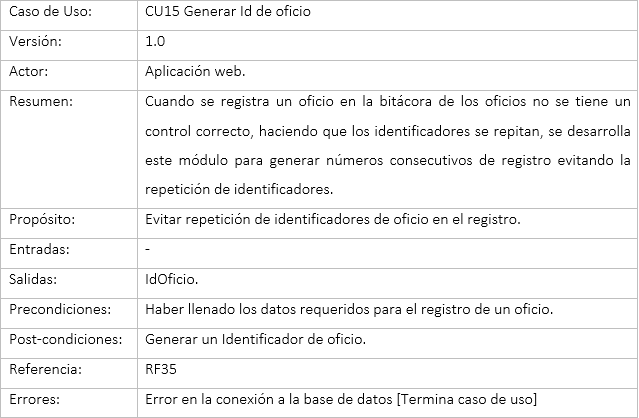
\includegraphics[width=0.8\textwidth]{images/CU/CU15}
		\caption{Caso de uso 15: Generar Id de oficio.}
		\label{Tabla}
	\end{figure}
	
\begin{itemize}
	\item Trayectoria principal:
	\begin{enumerate}
		\item 	La aplicación web hace una consulta a la base de datos solicitando el último id de oficio registrado.
\item	La aplicación genera el siguiente Id consecutivo.
\item	La aplicación regresa al CU origen. 
\item	Termina caso de uso.

	\end{enumerate}
	
\end{itemize}

%%%%%%%%%%%%%%%%%%%%%%%%%%%%%%%%%%%%%%%%%%%%%%%%%%%%%%%%%%%%%%%%%%%%%%%%%%%%
		\subsubsection{CU16: Consultar correspondencia por identificador}
\begin{figure}[htbp!]
		\centering
			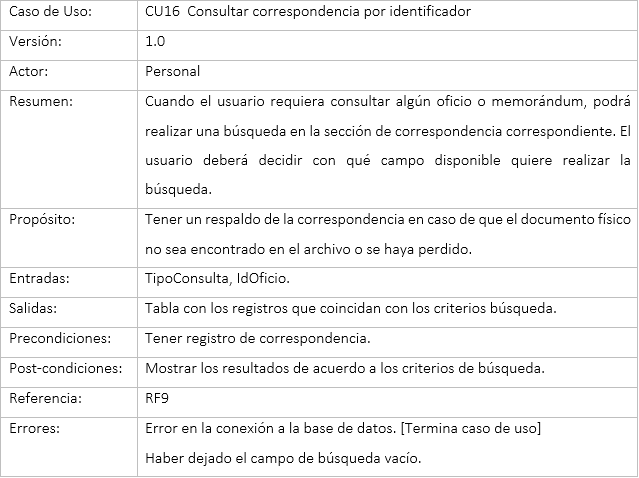
\includegraphics[width=0.8\textwidth]{images/CU/CU16}
		\caption{Caso de uso 16: Consultar correspondencia por identificador.}
		\label{Tabla}
	\end{figure}
	
\begin{itemize}
	\item Trayectoria principal:
	\begin{enumerate}
		\item	El actor va a la sección de oficios entrantes.
		\item	A través de los menús da clic en el tipo de correspondencia que desea consultar.
		\item	La aplicación muestra la pantalla \IUref{IU4} de Correspondencia correspondiente.
		\item	El actor ingresa el valor la categoría para la búsqueda.
		\item	El actor selecciona por qué campo desea realizar la búsqueda.
		\item	El actor presiona el botón “Buscar”.
		\item	La aplicación valida que el campo de criterio de búsqueda no esté vacío.
		\item	La aplicación realiza la consulta en la base de datos.
		\item	La aplicación muestra el mensaje \IUref{MSG6} de operación exitosa.
		\item	La aplicación muestra los resultados en una tabla.
		\item	Fin del caso de uso
	\end{enumerate}
	
	\item Trayectorias alternativas:
	\begin{itemize}
		\item Trayectoria alternativa A: Si está vacío el criterio de búsqueda.
			\begin{enumerate}
				\item La aplicación resalta el campo de criterio de búsqueda.
				\item Continúa en trayectoria principal en paso 4.
			\end{enumerate}
	\end{itemize}
\end{itemize}

%%%%%%%%%%%%%%%%%%%%%%%%%%%%%%%%%%%%%%%%%%%%%%%%%%%%%%%%%%%%%%%%%%%%%%%%%%%%
		\subsubsection{CU17: Consultar correspondencia por fecha de emisión}
\begin{figure}[htbp!]
		\centering
			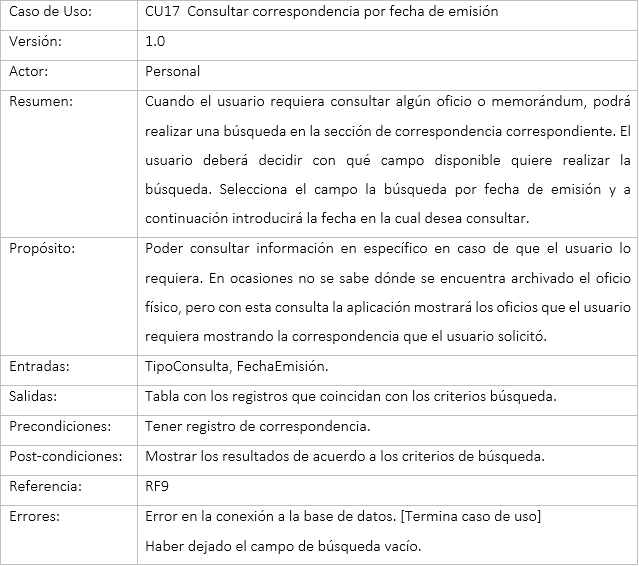
\includegraphics[width=0.8\textwidth]{images/CU/CU17}
		\caption{Caso de uso 17: Consultar correspondencia por fecha de emisión.}
		\label{Tabla}
	\end{figure}
	
\begin{itemize}
	\item Trayectoria principal:
	\begin{enumerate}
		\item	El actor va a la sección de oficios entrantes.
		\item	A través de los menús da clic en el tipo de correspondencia que desea consultar.
		\item	La aplicación muestra la pantalla \IUref{IU4} de Correspondencia correspondiente.
		\item	El actor ingresa el valor la categoría para la búsqueda.
		\item	El actor selecciona por qué campo desea realizar la búsqueda.
		\item	El actor presiona el botón “Buscar”.
		\item	La aplicación valida que el campo de criterio de búsqueda no esté vacío.
		\item	La aplicación realiza la consulta en la base de datos.
		\item	La aplicación muestra el mensaje \IUref{MSG6} de operación exitosa.
		\item	La aplicación muestra los resultados en una tabla.
		\item	Fin del caso de uso
	\end{enumerate}
	
	\item Trayectorias alternativas:
	\begin{itemize}
		\item Trayectoria alternativa A: Si está vacío el criterio de búsqueda.
			\begin{enumerate}
				\item La aplicación resalta el campo de criterio de búsqueda.
				\item Continúa en trayectoria principal en paso 4.
			\end{enumerate}
	\end{itemize}
\end{itemize}

%%%%%%%%%%%%%%%%%%%%%%%%%%%%%%%%%%%%%%%%%%%%%%%%%%%%%%%%%%%%%%%%%%%%%%%%%%%%
\subsubsection{CU18: Consultar correspondencia por emisor}
\begin{figure}[htbp!]
		\centering
			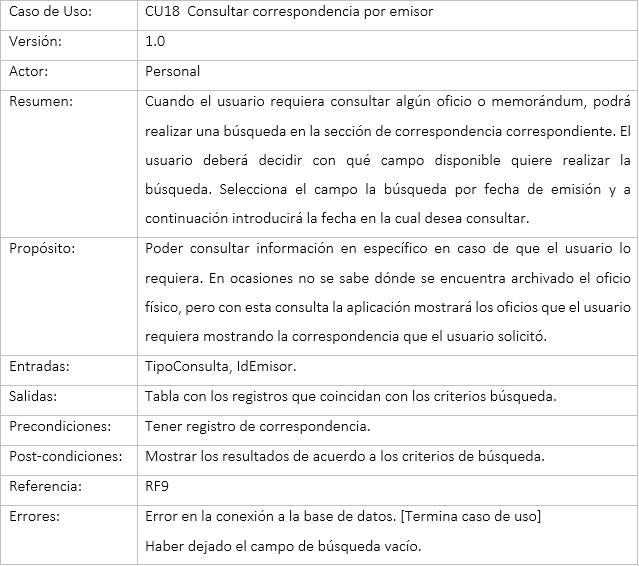
\includegraphics[width=0.8\textwidth]{images/CU/CU18}
		\caption{Caso de uso 18: Consultar correspondencia por emisor.}
		\label{Tabla}
	\end{figure}
	
\begin{itemize}
	\item Trayectoria principal:
	\begin{enumerate}
		\item	El actor va a la sección de oficios entrantes.
		\item	A través de los menús da clic en el tipo de correspondencia que desea consultar.
		\item	La aplicación muestra la pantalla \IUref{IU4} de Correspondencia correspondiente.
		\item	El actor ingresa el valor la categoría para la búsqueda.
		\item	El actor selecciona por qué campo desea realizar la búsqueda.
		\item	El actor presiona el botón “Buscar”.
		\item	La aplicación valida que el campo de criterio de búsqueda no esté vacío.
		\item	La aplicación realiza la consulta en la base de datos.
		\item	La aplicación muestra el mensaje \IUref{MSG6} de operación exitosa.
		\item	La aplicación muestra los resultados en una tabla.
		\item	Fin del caso de uso
	\end{enumerate}
	
	\item Trayectorias alternativas:
	\begin{itemize}
		\item Trayectoria alternativa A: Si está vacío el criterio de búsqueda.
			\begin{enumerate}
				\item La aplicación resalta el campo de criterio de búsqueda.
				\item Continúa en trayectoria principal en paso 4.
			\end{enumerate}
	\end{itemize}
\end{itemize}

%%%%%%%%%%%%%%%%%%%%%%%%%%%%%%%%%%%%%%%%%%%%%%%%%%%%%%%%%%%%%%%%%%%%%%%%%%%%

\subsubsection{CU19: Cancelar proceso de correspondencia}
\begin{figure}[htbp!]
		\centering
			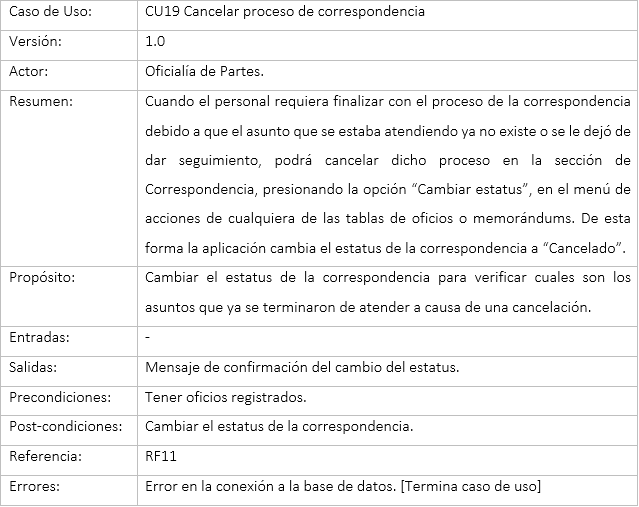
\includegraphics[width=0.8\textwidth]{images/CU/CU19}
		\caption{Caso de uso 19: Cancelar proceso de correspondencia.}
		\label{Tabla}
	\end{figure}
	
\begin{itemize}
	\item Trayectoria principal:
	\begin{enumerate}
		\item El actor va a la sección de correspondencia.
		\item	La aplicación muestra la pantalla \IUref{IU21} Correspondencia saliente.
		\item	CU16, CU17 o CU18 Consultar correspondencia.
		\item	El actor presiona el botón “Acciones” de la correspondencia a cancelar.
		\item	El actor selecciona la opción “Cancelar oficio” o “Cancelar memorándum”.
		\item	La aplicación cambia el estatus de la correspondencia en la base de datos.
		\item	La aplicación muestra el mensaje MSG5 de que el cambio de estatus se ha llevado a cabo de forma correcta.
\item	Termina caso de uso.

	\end{enumerate}
\end{itemize}

%%%%%%%%%%%%%%%%%%%%%%%%%%%%%%%%%%%%%%%%%%%%%%%%%%%%%%%%%%%%%%%%%%%%%%%%%%%%
